To evaluate the in-sample and out-of-sample performances of the models described by (Contreras-Espinoza et al., 2023), a time series of new daily infections of COVID-19 in the area served by the main Bologna WWTP, from October 13, 2021, to April 4, 2023 ($T = 539$ observations) is used. \\

Table \ref{tab:descr_stat} presents the data summary statistics, the $p$-value of the Jarque–Bera (JB) test (Jarque \& Brera, 1980) and the $p$-value of the augmented Dickey–Fuller (ADF) test (Dickey \& Fuller, 1979). For the JB test, the null hypothesis of normal distribution is rejected at the 1\% significance level. This supports the use of the negative binomial distribution for the score-driven model. For the ADF test, the null hypothesis that a unit root is present in the time series cannot be rejected, which supports using the unit root specifications for $\delta_t$ in Equations (3) and (11). These results are aligned with those obtained by (Contreras-Espinoza et al., 2023) for nine Latin American countries, justifying the use of the data regarding new daily infections of COVID-19 in the area served by the main Bologna WWTP to evaluate (Contreras-Espinoza et al., 2023) models' performance.\\

\begin{table}[h!]
\centering
\caption{Descriptive statistics, JB test, and ADF test for new COVID-19 cases}
\centering
\renewcommand{\arraystretch}{1.5}
\begin{tabular}[h]{c c c c}
\hline
\textbf{Mean} & \textbf{Std. Dev.} & \textbf{Minimum} & \textbf{Maximum} \\
\hline
354.264 & 413.413 & 13 & 2659 \\
\hline
& & & \\
\hline
\textbf{Skewness} & \textbf{Kurtosis} & \textbf{JB \textit{p}-value} & \textbf{ADF \textit{p}-value} \\
\hline
2.631 & 11.139 & 0.000 & 0.055\\
\hline
\end{tabular}
\label{tab:descr_stat}
\end{table}
\vspace{0.4cm}

For the full sample period, parameter estimates for SD1, SD2, SDWS, and SS are reported in Table \ref{tab:parameters}. The parameters $\kappa_1$ and $\kappa_2$ are significant in both SD1, SD2 and SDWS, indicating that the local level ($\delta_t$) and trend ($\beta_t$) components are crucial for these models. Moreover, the estimates are relatively consistent, suggesting robustness in capturing the core dynamics of the data. \\

Looking at the seasonal parameters of SD1 ($\kappa_{j,t}$ where $j \in \{\text{Monday, Tuesday, } \dots\text{, Sunday}\}$, a significant effect of Mondays emerged. This might capture weekly patterns in reporting case numbers, reflecting some regularity in data collection or transmission cycles. Also $\kappa_{\text{Saturday}}$ and $\kappa_{\text{Sunday}}$ are significant, suggesting a potential weekend effect on the data, likely due to reporting delays. The seasonality parameter $\kappa$ is also significant for SD2, confirming the presence of a weekly seasonal trend in the data.\\

The dispersion parameter of the negative binomial distribution ($\nu$) is significant across all models. The values vary widely, with the highest being in the SS model (72.6) and the lowest in the SDWS model (9.30). This indicates different levels of over-dispersion captured by each model. \\

\begin{table}[t!]
\centering
\begin{threeparttable}
\caption{Parameter estimates}
\centering
\renewcommand{\arraystretch}{1.5}
\begin{tabular}[h]{l r r r r } 
\hline
 & \textbf{SD1} & \textbf{SD2} & \textbf{SDWS} & \textbf{SS} \\
 \hline
 $\kappa_1$ & 0.408 *** (0.030) & 0.391 *** (0.029) & 0.196 *** (0.017) & -\\
 $\kappa_2$ & 0.074 *** (0.010) & 0.070 *** (0.010) & 0.053 *** (0.006) & -\\
 $\kappa_{\text{Monday}}$ & 0.169 *** (0.063) & 0.111 *** (0.019) & - & -\\
 $\kappa_{\text{Tuesday}}$ & 0.000 (0.000) & - & - & -\\
 $\kappa_{\text{Wednesday}}$ & 0.000 (0.000) & - & - & -\\
 $\kappa_{\text{Thursday}}$ & 0.000 (0.000) & - & - & -\\
 $\kappa_{\text{Friday}}$ & 0.000 (0.000) & - & - & - \\
 $\kappa_{\text{Saturday}}$ & 0.103 ** (0.041) & - & - & - \\
 $\kappa_{\text{Sunday}}$ & 0.228 *** (0.056) & - & - & -\\
 $\nu$ & 38.2 *** (2.76) & 35.3 *** (2.62) & 9.30 *** (0.60) & 72.6 *** (8.83)\\
 $\sigma^2_{\beta}$ & - & - & - & 0.0000 (0.001)\\
 $\sigma^2_{\delta}$ & - & - & - & 0.0002 *** (0.000)\\
 $\sigma^2_{\gamma}$ & - & - & - & 0.0001 *** (0.000)\\
\hline
\end{tabular}
\label{tab:parameters}
\begin{tablenotes}
\footnotesize
\item \textit{Notes}:  Standard errors are in parentheses. ***, **, and * indicate parameter significance at the 1\%, \\ \hspace{2em} 5\%, and 10\% levels, respectively. For SD2, $\kappa_j = \kappa_{\text{Monday},t}$ for $j = \text{Tuesday}, \dots , \text{Sunday}$. 
\end{tablenotes}
\end{threeparttable}

\end{table}

The variance components of the SS model ($\sigma^2_{\beta}$, $\sigma^2_{\gamma}$, $\sigma^2_{\delta}$) are all significant. This suggests that the SS model explicitly accounts for additional sources of variability. Even though the estimates are very small, the inclusion of these components could explain the higher $\nu$ value and reflect a greater adaptability to data variations. \\

In Figures 1-4, for each of the four models tested, the filtered estimates of new cases of infection with COVID-19 are represented together with the observed time series. SD1, SD2 and SS appear to have similar performance, with the estimates (red lines) and observed data (black lines) showing close alignment across the time series. Both models show some deviations at the peaks but generally capture the overall trend series well. SDW instead seems to capture only the overall trend of the series, with less accuracy in capturing the sharp fluctuations in the data. This suggests that the SDWS model may not be as reliable in terms of prediction accuracy.\\

\begin{figure}
\centering
\begin{subfigure}{\textwidth}
\caption{Filtered estimates of new cases of infection with COVID-19 (SD1)}
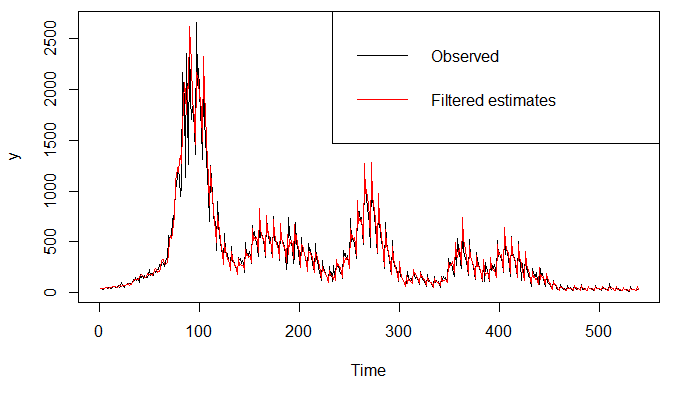
\includegraphics[width=0.95\textwidth, inner]{SD1_plot.png}
\label{fig:SD1}
\end{subfigure}
\begin{subfigure}
    \caption{Filtered estimates of new cases of infection with COVID-19 (SD2)}
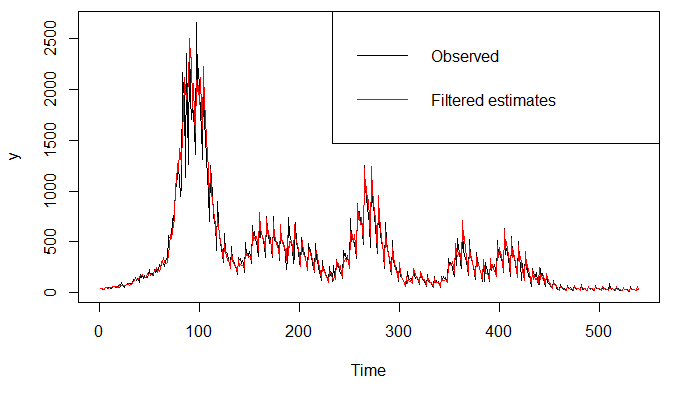
\includegraphics[width=0.95\textwidth, inner]{SD2_plot.png}
\label{fig:SD2}
\end{subfigure}
\end{figure}

\begin{figure}
\centering
\begin{subfigure}{\textwidth}
\caption{Filtered estimates of new cases of infection with COVID-19 (SDWS)}
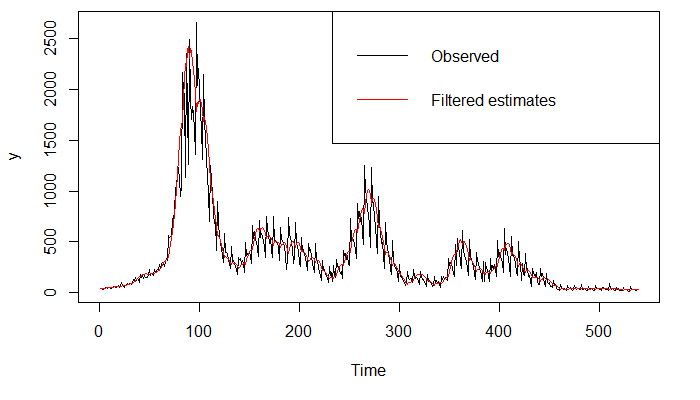
\includegraphics[width=0.95\textwidth, inner]{SDWS_plot.png}
\label{fig:SD1}
\end{subfigure}
\begin{subfigure}
    \caption{Filtered estimates of new cases of infection with COVID-19 (SS)}
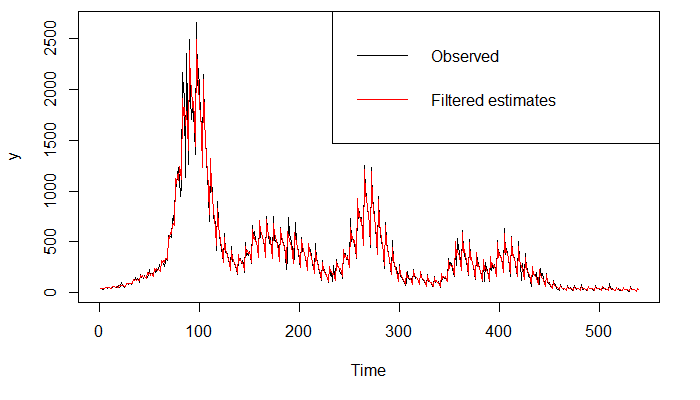
\includegraphics[width=0.95\textwidth, inner]{SS_plot.png}
\label{fig:SD2}
\end{subfigure}
\end{figure}

To evaluate the predictive capacity of the SD1 SD2, SDWS and SS models, the same procedure used by (Contreras-Espinoza et al., 2023) was followed. First, the observed time series was divided into two equal parts (270 and 269 observations, since $T$=539). Considering a 7-day prediction window, the last 7 observations were removed from the initial half of the data and predicted using the remaining data and the parameters presented in Table \ref{tab:parameters}. The metrics described in sections 2.6 and 2.7 were calculated to evaluate statistical performance and predictive capacity of the fitted models. Then, the next observation (observation 271) was included in the fitting data. The last 7 observations were again removed and predicted using parameters in Table \ref{tab:parameters}, and the prediction quality was evaluated. These steps were repeated until the total set of available observations was considered. Finally, the same procedure was repeated using 14- and 28-day time windows. \\

Tables \ref{tab:7d}, \ref{tab:14d} and \ref{tab:28d} show the mean values of AIC, AICc, BIC, MSE, MAE, and MAPE for the different models considering 7-, 14- and 28-day estimation windows, respectively. SD2  has the best performance in terms of AIC, AICc and BIC, suggesting it is the best model when it comes to considering the trade-off between model complexity and fit. SD1 has instead the lowest prediction accuracy metrics for all three forecasting windows tested (the best values have been highlighted in bold). SDWS seems to be the least preferred model among those tested due to poorer fit and prediction accuracy. Furthermore, when the size of the forecasting window increases, the prediction quality of all models decreases: for example, the SD1 MAPE value is 22.5\% for the 7-day forecast, 34\% for the 14-day forecast and 75.54\% for the 28-day forecast. \\
\textcolor{white}{________________}

\begin{table}[h!]
\centering
\caption{AIC, AICc, BIC, and loss functions (forecasting window: 7 days)}
\centering
\renewcommand{\arraystretch}{1.5}
\begin{tabular}[h!]{l c c c c c c}
\hline
\textbf{Model} & \textbf{AIC} & \textbf{AICc} & \textbf{BIC} & \textbf{MSE} & \textbf{MAE} & \textbf{MAPE}\\
\hline
SD1 & 4280.132 & 4281.999 & 4351.690 & \textbf{3909.353} & \textbf{37.188} & \textbf{0.225}\\
SD2 & \textbf{4258.316} & \textbf{4259.165} & \textbf{4305.881} & 5335.746 & 41.948 & 0.227\\
SDWS & 4713.311 & 4713.471 & 4733.130 & 14474.359 & 73.161 & 0.417\\
SS & 4298.022 & 4298.129 & 4313.878 & 5927.632 & 43.523 & 0.232\\
\hline
\end{tabular}
\label{tab:7d}
\end{table}\\


\begin{table}[h!]
\centering
\caption{AIC, AICc, BIC, and loss functions (forecasting window: 14 days)}
\centering
\renewcommand{\arraystretch}{1.5}
\begin{tabular}[h!]{l c c c c c c}
\hline
\textbf{Model} & \textbf{AIC} & \textbf{AICc} & \textbf{BIC} & \textbf{MSE} & \textbf{MAE} & \textbf{MAPE}\\
\hline
SD1 & 4249.468 & 4251.349 & 4320.880 & \textbf{14365.77} & \textbf{61.953} & \textbf{0.340}\\
SD2 & \textbf{4196.611} & \textbf{4197.475} & \textbf{4243.972} & 22533.51 & 74.646 & 0.348\\
SDWS & 4642.673 & 4642.836 & 4662.407 & 41193.64 & 109.529 & 0.568\\
SS & 4236.084 & 4236.192 & 4251.871 & 32032.90 & 84.559 & 0.383\\
\hline \\
& & & & & & \\
\end{tabular}
\label{tab:14d}
\end{table} \\

\begin{table}[h!]
\centering
\caption{AIC, AICc, BIC, and loss functions (forecasting window: 28 days)}
\centering
\renewcommand{\arraystretch}{1.5}
\begin{tabular}[h]{l c c c c c c}
\hline
\textbf{Model} & \textbf{AIC} & \textbf{AICc} & \textbf{BIC} & \textbf{MSE} & \textbf{MAE} & \textbf{MAPE}\\
\hline
SD1 & 4186.649 & 4188.560 & 4257.766 & \textbf{138410.9} & \textbf{140.267} & \textbf{0.754}\\
SD2 & \textbf{4060.468} & \textbf{4061.370} & \textbf{4107.371} & 214083.7 & 192.565 & 0.814\\
SDWS & 4486.913 & 4487.083 & 4506.456 & 508463.8 & 264.977 & 1.252\\
SS & 4099.487 & 4099.600 & 4115.121 & 929847.5 & 329.825 & 1.387\\
\hline \\
& & & & & & \\
\end{tabular}
\label{tab:28d}
\end{table}
